
\documentclass[journal,UTF8]{IEEEtran}
%\usepackage{ctex}
\usepackage{color}

%
\usepackage{cite}

\ifCLASSINFOpdf
 \usepackage[pdftex]{graphicx}
  % declare the path(s) where your graphic files are
 \graphicspath{{../pdf/}{../jpeg/}}
  % and their extensions so you won't have to specify these with
  % every instance of \includegraphics
\DeclareGraphicsExtensions{.pdf,.jpeg,.png}
\else
  % or other class option (dvipsone, dvipdf, if not using dvips). graphicx
  % will default to the driver specified in the system graphics.cfg if no
  % driver is specified.
\usepackage[dvips]{graphicx}
  % declare the path(s) where your graphic files are
\graphicspath{{../eps/}}
  % and their extensions so you won't have to specify these with
  % every instance of \includegraphics
\DeclareGraphicsExtensions{.eps}
\fi

\usepackage[cmex10]{amsmath}

%\usepackage{algorithmic}
\usepackage[ruled]{algorithm2e}
\usepackage{array}

\ifCLASSOPTIONcompsoc
  \usepackage[caption=false,font=normalsize,labelfont=sf,textfont=sf]{subfig}
\else
  \usepackage[caption=false,font=footnotesize]{subfig}
\fi

\hyphenation{op-tical net-works semi-conduc-tor}



\begin{document}
%
% paper title
% can use linebreaks \\ within to get better formatting as desired
% Do not put math or special symbols in the title.
\title{A VCA Protocol Based Multi-level Flexible Architecture on Embedded PLCs for Visual Servo Control }

\maketitle


\begin{abstract}

% ^.
\end{abstract}

% Note that keywords are not normally used for peerreview papers.
\begin{IEEEkeywords}
motion control, visual servo control, embedded PLC, multi-level architecture
\end{IEEEkeywords}

% For peer review papers, you can put extra information on the cover
% page as needed:
% \ifCLASSOPTIONpeerreview
% \begin{center} \bfseries EDICS Category: 3-BBND \end{center}
% \fi
%
% For peerreview papers, this IEEEtran command inserts a page break and
% creates the second title. It will be ignored for other modes.
\IEEEpeerreviewmaketitle



\section{Introduction}
Integration technologies is driving the industrial automation \cite{Kazmierkowski2007Integration}. The continuously integrations of sensors, controllers, robots, tools, etc. bring the concepts of self-aware equipment, intelligent factory and CPS, etc. \cite{Wan2018An,Chekired2018Industrial}.  Recent researches \cite{Colombo2006An,Vaccaro2010An,Dean2017Integration} introduce the development of integration technologies. In industrial automation, logic control system,  motion control system and visual system become more and more important and inseparable \cite{Feng2002Integrating,Chang2006Motion,Feng2005Practical}. On the other hand, the advances of edge computing, fog computing and edge artificial\cite{Hu2017Fog,Hou2018Green,PaceAn} put forward new challenges on edge equipment.

\subsection{Motivations}
%Nowdays, visual system has been applied in various fields.
%
%On the other hand, according to the reliablity and \cite{Hossain2014Advanced}, Lots of papers are focusing on it, \cite{Jiang2013System,Jiang2013Bayesian} guarantee the reliability by verifying the program of PLCs, \cite{Gerk2006Advanced,Chang2007Adaptive,Dominic2016PLC} improve the performance of PLCs using advanced algorithms, \cite{wu2018customized} alleviates the development complexity of PLCs with a special software structure, \cite{Sch2013Development,Morenas2017Shop} pose methods to update PLC programs dynamically.
%
%Motion control is a key technology\cite{Ohnishi2002Motion} of automation. It drives various types of equipments to replace tremendous labors. Since advanced in algorithms, in
Nowdays, visual system has been applied in various fields. The logic control on PLC has wide applications. Motion control 
\cite{Chen2014A} is a typical case that describes how the three parts collaborate. The visual system analyzes the context and get error put into the motion system. Simultaneously the logic program are judging the information, such as the position limitation of the every axis. Hence, how to pose a flexible structure to the integration of logic control system, servo system and visual system, guides us.





\subsection{Related Works}

Visual control system is combined of special motion control system and visual system. Such as transport \cite{Xing2014Intersection}, circuit detection\cite{Nian2005An}, sorting system, welding\cite{Chen2014A}, assembling\cite{Wang2008Visual,Xiao2014Visual}, robot\cite{Wu2013Cloud,Tsai2017A}, unmanned aerial vehicles\cite{Guenard2010A,Serra2016Landing}. These works address their problems in relevant fields. However, all these solutions are based on special motion control system and visual system.

%例如\cite{Wu2013Cloud,Tsai2017A}中均使用机器人专用控制系统和视觉系统完成,在\cite{Guenard2010A,Serra2016Landing}中,使用无人机专用控制系统和视觉系统完成。\cite{Nian2005An}中,通过专用运动控制卡和视觉系统实现电路检测。

On the other hand. The integration of logic control and motion control has variously deep researches \cite{Ioannides2004Design,Shi2016The,Fang2017Design, syaichu2011model}. \cite{Ioannides2004Design,syaichu2011model} realize the motion control directly in PLC. \cite{Peng2011Linear, Qian2014A, OMRON2006CS1W} use motion control module collaborated with PLC to implement their applications. However, the development method in these papers is disordered. Therefore, in 2005, PLCopen organization has released a related standard \cite{PLCopen2005Function} which standardizes the motion control in PLC. Based on this standardization, \cite{S2006Advanced} provides an advanced implementation in distributed automation system and companies, such as 3S \cite{3S2017Logic}, provide some tools. \cite{wu2018customized} poses a customized real-time compilation method to reduce the development complexity.

Above works provide impressive integrations on visual servo control system and PLC with motion control functions, however there are few papers discussing the integration of visual system, motion control and PLC. Most of applications are focusing on its application with three individual system, such as \cite{Chen2014A}. Hence, an integration structure of logic control system, servo system and visual system should be provided to reduce the complexity and expand the application fields.

\subsection{Our Contributions}
.
%我们提出了一种基于VCA协议的ePLC和视觉系统的柔性架构整合方案,来实现视觉私服控制。VCA协议描述了从视觉系统中获取数据后的组帧和在ePLC中数据帧在各层中的解析,从而实现视觉系统和ePLC的整合。ePLC硬件上的一种定制化设计,软件架构上的三层设计以及融合其中的VCA协议使得整个视觉私服系统变成一种柔性结构。
%
%在接下来的部分中,\ref{SystemStructure}会介绍系统组成,包括硬件结构,软件结构,线程结构和内存设计。\ref{Integration}会介绍ePLC如何与视觉系统融合,包括VCA协议,PLC接口和视觉接口介绍。\ref{Execution}介绍系统执行过程,包括视觉层执行过程,逻辑层执行过程,算法层执行过程和多线程执行。\ref{Case}中介绍了两个例子,带视觉检测的绕线机和双目接球机器人。

\section{System Architecture}
\label{SystemStructure}
\subsection{Hardware Structure}
The hardware is comprised of ePLC system ($ES$)and visual system ($VS$). The $ES$ is a customized structure. The number of DI/DO, AI/AO and controlled servo system could be increased according to applications. Fig. \ref{fig:Hardware} shows a typical $ES$ which adopts two processor architecture. The shared memory is used to transfer data between master and slave processors. The communication between $ES$ and $VS$ could adopt multiple protocols, such as TCP, modbus, CAN, etc. In the shown Fig. \ref{fig:Hardware}, we adopt the CAN Bus.

\begin{figure}
	\centering
	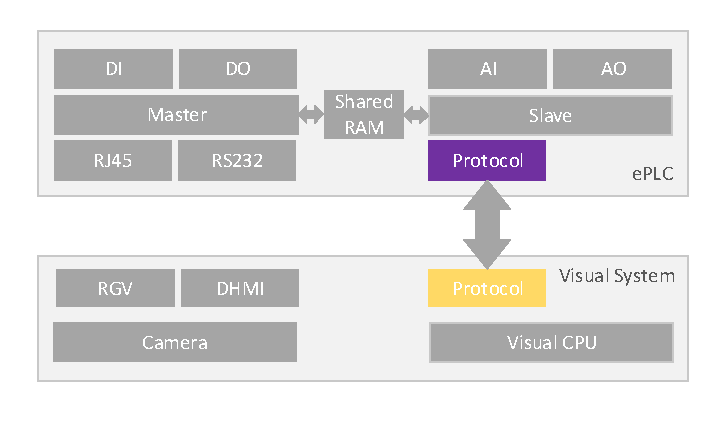
\includegraphics[width=3.5in]{fig/Hardware.pdf}
	\caption{A typical $ES$ which adopts two processor architecture. The shared memory is used to transfer data between master and slave processors. The communication between $ES$ and $VS$ adopt the CAN Bus.}
	\label{fig:Hardware}
\end{figure}
\subsection{Software Structure}
In normal visual control system, the typical software structure is seen as in the left of Fig. \ref{fig:Software}.
To our best knowledge, the $VS$ contains several visual algorithms and every algorithm could extract some required parameters form pictures or videos. Meanwhile, the $ES$ is comprised of modules which conclude logic part and algorithms and algorithms here are main motion control algorithms. Regarding the normal development method of visual servo control, the $VS$ and $ES$ is developed individually and using the communication protocol combines this two parts. However, this method should be always redesigned the programs in both systems because of the various visual algorithms and motion control algorithms. In addition, the logic and motion control are mixed together to develop in $ES$ and there are also lots of communication protocols (EtherCat, Modbus, Can, etc.). Considering the high complexity of today’s applications, it will be a cumbersome task.

Hence, we propose a multi-level flexible architecture which is based on $VCA$ protocol. As shown in Fig. \ref{fig:Software}, the architecture contains three layers: flexible layer ($FL$), control layer ($CL$) and algorithm layer ($AL$).

\textbf{Flexible layer}: these layer is responsible for joint the $VS$ and $ES$ and consists of $PLC$ interface and visual interface. The parameters are framed with $VCA$ protocol frame (henceforth
, abbreviated form of $PF$) interacted between $VS$ and $ES$. Furthermore, a special protocol template ($PT$) is saved in both systems to illustrate the protocol.

\textbf{Control layer}: this is independent of algorithm layer to cope with the logic tasks. This make it possible to run the logic task and algorithm task in different processors.

\textbf{Algorithm layer}: it is mainly comprised of types of algorithms which could be built in individual processors for algorithms with high performance requirement. 


\begin{figure}
	\centering
	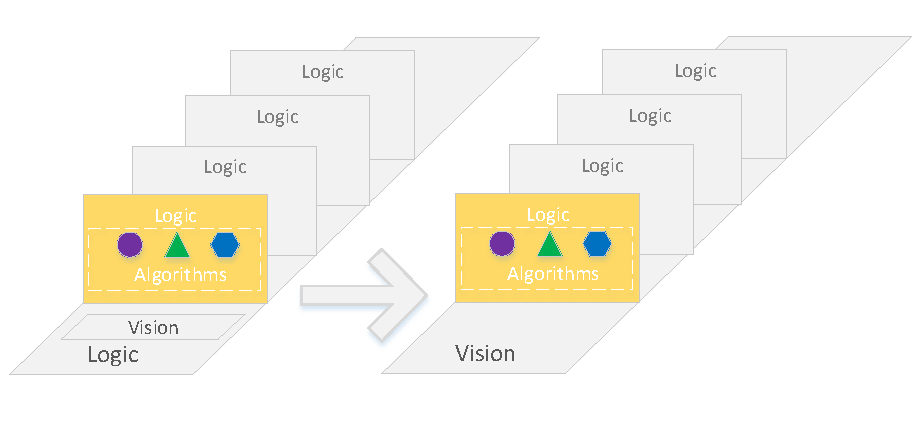
\includegraphics[width=3.5in]{fig/Software.pdf}
	\caption{Multi-level flexible architecture contains three layers: flexible layer, control layer and algorithm layer.}
	\label{fig:Software}
\end{figure}
%%%Fig.4. The three-layer architecture of embed PLC.



\subsection{Thread Structure}
We adopt the analogous thread structure in \cite{wu2018customized}. Three special threads introduced below:
\begin{enumerate}
	\item Visual Thread. This thread is responsible for interaction with $VS$. It will receive the protocol frame from the $VS$ and save it to relevant address. 
	\item Control Thread. Control thread mainly execute logic program, deframe the protocol frame and interaction data with algorithm thread.
	\item Algorithm Thread. Algorithm thread runs in slave processors. It is used to implement data interaction between processors and execution of algorithms.
\end{enumerate}

\begin{figure}
	\centering
	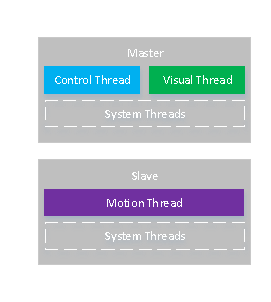
\includegraphics[width=3in]{fig/Threads.pdf}
	\caption{ Thread structureThe with three special threads: visual thread, Control thread, algorithm thread.}
	\label{fig:Threads}
\end{figure}
\subsection{Memory Allocation}
\begin{figure}
	\centering
	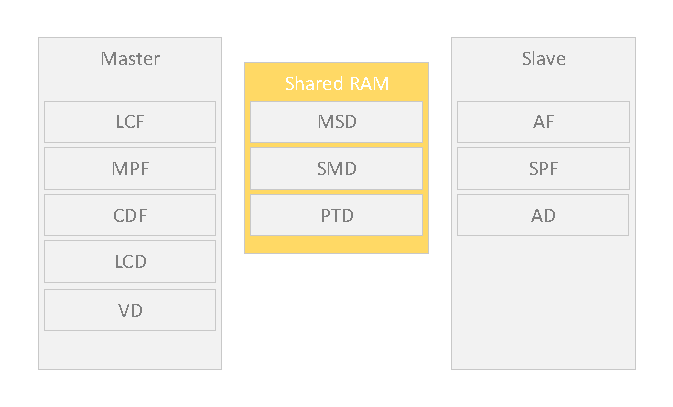
\includegraphics[width=3in]{fig/RAM.pdf}
	\caption{Memory allocation of master processor, shared ram and slave processor.}
	\label{fig:RAM}
\end{figure}
The dedicated storage area of $PLC$ in memory is made up of bit data area ($M$ area) and byte data area ($D$ area). Meanwhile, we regard $M$ area and $D$ area as set $M$ of bit and set $D$ of byte. Henceforth, we have three definitions below.

\textbf{Definition 1} If $\exists$ set $S$, we define its subscripted lowercase letter $s_i$ as an element of $S$ and the subscripted $i$ is used to distinguish the elements.

\textbf{Definition 2} If $\exists S \subseteq M$ and $(\forall s_{i} \in S) \in \{0, 1\} $. Meanwhile, each element $s_i$ has four operators: $\mathcal{S}_0(s_i)$ assigns $0$ to $s_i$, $\mathcal{S}_1(s_i)$ assigns $1$ to $s_i$, $\mathcal{J}_0(s_i)$ represents that the value of $s_i$ is $0$, $\mathcal{J}_1(s_i)$ means that the value of $s_i$ is $1$. Then we define the set $S$ has $\mathcal{B}$ attribute.

\textbf{Definition 3} If $\exists S \subseteq D$ and $\forall s_{i} \in S$ has 4 bytes. We define the set $S$ has $\mathcal{D}$ attribute.

Fig. \ref{fig:RAM} shows the memory allocation of master processor, shared RAM and slave processor. The shared $RAM$ is a special structure to fast data interaction between master and slave processors. In more general cases, the $MtoS$ is located in master processor, the $StoM$ is located in slave processor and the $PT$ is in both master and slave processors. 

\textbf{\emph{LCF}} (Logic Control Flag Area): the flag are used to start the modules. It has $\mathcal{B}$ attribute.

\textbf{\emph{MPF}} (Master Processor Data Interaction Flag Area): it contains begin data transfer flag from master to slave ($MSB$), transfer state of master from master to slave ($MSF$), acknowledge flag of master from master to slave ($MSA$) and transfer state of master from slave to master ($MSS$). All of them have $\mathcal{B}$ attribute.


\textbf{\emph{CDF}} (control frame saved flag area): this flags denote whether the control frame is saved. It has $\mathcal{B}$ attribute.

\textbf{\emph{LCD}} (Logic Control Data Area): these data will be used to store the control frame. It has $\mathcal{D}$ attribute. Every element $lcd_i$ is associated with a specified module.

\textbf{\emph{VD}} ($VCA$ protocol frame data area): all the frames received from the $VS$ are stored in this area.

\textbf{\emph{MSD}} (Master Processor Data Interaction Data Area): an area stores the data delivered from slave processors and it has $\mathcal{D}$ attribute.

\textbf{\emph{SMD}} (Slave Processor Data Interaction Data Area): an area stores the data delivered from master processor and it has $\mathcal{D}$ attribute.

\textbf{\emph{PTD}} (Protocol Template Data Area): the protocol template is stored in this area and could be read by both processors.


\textbf{\emph{AF}} (Algorithm Flag Area): it includes algorithm flag of execution ($AFE$) and algorithm flag of state ($AFS$).
Both of them have $\mathcal{B}$ attribute.

\textbf{\emph{SPF}} (Slave Processor Data Interaction Flag Area): this area includes the begin data transfer flag from slave to master ($SMB$), transfer state of slave from slave to master ($SMF$), acknowledge flag of slave from slave to master ($SMA$) and transfer state of slave from master to slave ($SMS$). All of them have $\mathcal{B}$ attribute.

\textbf{\emph{AD}} (Algorithm Data Area): these data help specified algorithm executing. It has $\mathcal{D}$ attribute.
 
 We define the $\mathcal{P}$ to interact data between master processor and slave processor. It contains transferring data from master to slave ($\mathcal{P}_{mts}$) and transferring data from slave to master ($\mathcal{P}_{stm}$) which is defined below:
 \begin{equation}
 \left\{
 \begin{array}{l}
 \mathcal{P}_{mts} = \mathcal{U} (msb_i,msf_i,sma_i,sms_i,smd_i)\\
 \mathcal{P}_{stm} = \mathcal{U} (smb_i,smf_i,msa_i,mss_i,msd_i)
 \end{array}
 \right.
 \end{equation}
 Where $\mathcal{U}$ is the function to implement the process of data interaction between master and slave processors. $\mathcal{P}_{mts}$ and $\mathcal{P}_{mts}$ use the same function $\mathcal{U}$.
 
 The process of $\mathcal{P}_{mts}$ is seen below:
 	$\mathcal{S}_1(msb_i)\to\mathcal{S}_1(msf_i)\to send(smd_i)\to\mathcal{S}_0(msb_i)\to\mathcal{S}_1(sms_i)\to check(smd_i)\to\mathcal{S}_1(sma_i)\to\mathcal{S}_0(sms_i)\to\mathcal{S}_0(sma_i)\to\mathcal{S}_0(msf_i)$.
 
 Where $send(msd_i)$ means sending data to $msd_i$ in slave processor. $check(msd_i)$ means to check data of $msd_i$.

 

%%%Fig.6. Distribution of dedicated public data area.
\section{Integration of $VS$ and $ES$}
\label{Integration}

\subsection{VCA Protocol Template}
\begin{figure}
\centering
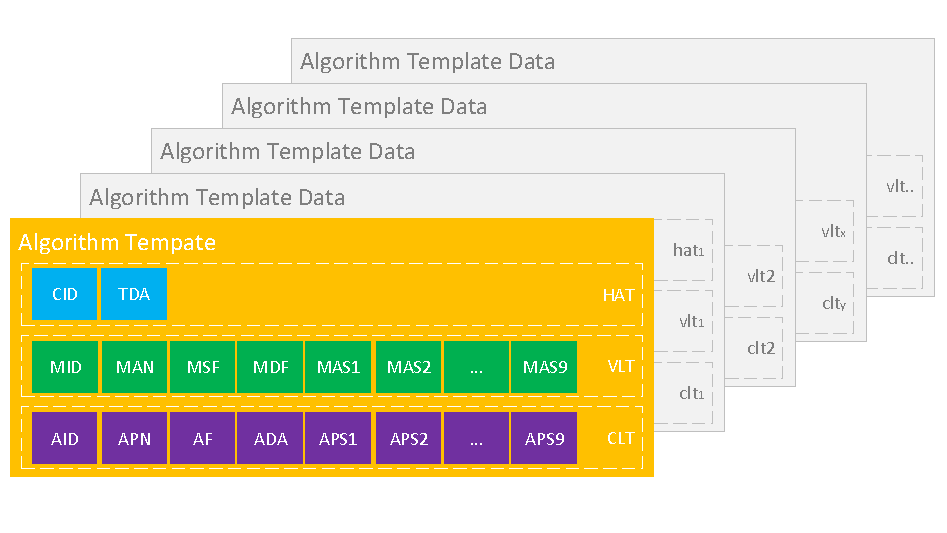
\includegraphics[width=3.5in]{fig/PT.pdf}
\caption{A $PT$ uniquely corresponds to a type of application. It contains four parts: head of protocol template, visual layer template , control layer template and algorithm layer template.}
\label{fig:PT}
\end{figure}
In cater to most applications, we propose a VCA-based multi-level flexible architecture. As shown in Fig. \ref{fig:PT}, a protocol template ($PT$) is adopted to support various types of implementations and a $PT$ uniquely corresponds to a type of application. In the flexible architecture, users only need to redesign and reload the $PT$ and then they can reuse the visual servo system again. The $PT$ could be loaded into a stationary address of visual system and ePLC system. After restarting both systems, it will be put into a fixed area of $RAM$. The parsing modules form both systems will read it when parsing the protocol data.
 
 The $PT$ is defined below:
 \begin{equation}
 \left\{
 \begin{array}{l}
    PT = \{HPT, VLT, CLT, ALT\}\\
    HPT = \{CID, TDA\}\\
    VLT = \{MID, MAN, MSF, MDA, MAS, CDATA\}\\
    CLT = \{AID, APN, AF, ADA, APS, ADATA\}\\
    ALT = \{PID, PDATA\}
 \end{array}
 \right.
 \end{equation}
 
 The $PT$ contains four parts: head of protocol template ($HPT$), visual layer template ($VLT$), control layer template ($CLT$) and algorithm layer template ($ALT$). Every part explains as follows: 
 \begin{enumerate}
 	\item $HPT$: this part includes communication unique ID ($CID$), template data storage address ($TDA$). Every $PT$ only has one $HPT$.
 	\item $VLT$: it consists of module unique ID ($MID$), module contained algorithm number ($MAN$), module start flag ($MSF$), module data start address ($MDA$), module contained algorithm IDs ($MAS$) . $VLT$ is not $\emptyset$. Every $MAS$ include $MAN$ algorithm IDs. 
 	\item $CLT$: it is comprised of algorithm unique ID ($AID$), algorithm contained parameter number ($APN$), $AF$, algorithm data start address $ADA$, algorithm contained parameter IDs ($APS$). $CLT$ is not $\emptyset$. Every $APS$ include $APN$ parameter IDs.
 	\item $ALT$: it contains parameter unique ID ($PID$). $ALT$ is not $\emptyset$. 
 \end{enumerate}
 \subsection{$VCA$ Protocol Frame}
 The $VCA$ protocol frame ($PF$) contains control frame and algorithm frame in its data field as shown in \ref{fig:Protocol}. 

 \begin{enumerate}
	\item $PF$: it consists items of $MID$, visual frame length $VFL$, $CDATA$ and cyclic redundancy check $CRC$.The $CDATA$ contains several control frames. The $MID$s both in $PT$ and $PF$ need one-to-one correspondence.
	\item Control frame: it is comprised of $AID$, control frame length ($CFL$) and $ADATA$.
	The $ADATA$ includes several algorithm frames. The $AID$s both in control frame and $PF$ need one-to-one correspondence.
	\item Algorithm frame: it contains $PID$, $PDATA$. $PID$ is also the address of $PDATA$. The $PID$s both in algorithm frame and $PF$ need one-to-one correspondence.
\end{enumerate}


\begin{figure}
	\centering
	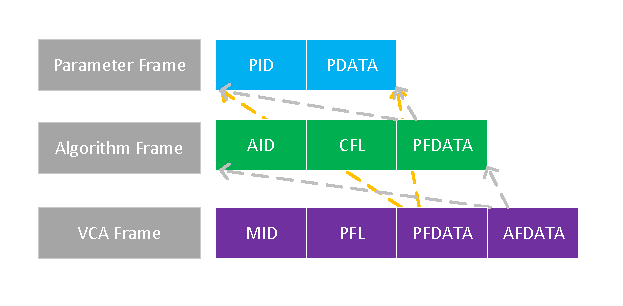
\includegraphics[width=3in]{fig/Protocol.pdf}
	\caption{ $VCA$ protocol frame contains control frame and algorithm frame in its data field.}
	\label{fig:Protocol}
\end{figure}
\subsection{Framing of $PF$}
In $VS$, the $PLC$ interface will frame the $PF$ and transfer it to $PLC$. The framing contains three steps: $VCA$ framing, $CL$ framing, $AL$ framing.


\textbf{\emph{VCA} Framing}: the process is realized as the Algorthm \ref{alg1}. It searches the $PT$ with $mid$ to find the relevant $vlt_x$. Through it, the $VS$ can obtain the $msf$ and $mda$. According to $man$, call the next step ($VL$ Framing) to gain the $cdata$. Then calculate the length ($vfl$) and $crc$ to finish the $VL$ framing.

\textbf{\emph{CL} Framing}: Algorthm \ref{alg2} illustrates the process. The $VS$ seeks the $FT$ to gain the $clt_y$ which contains the $af$ and $ada$. According to $apn$, call the next step ($AL$ Framing) to obtain the $cdata$ and then calculate the length ($cfl$) to finish the $CL$ framing.  

\textbf{\emph{AL} Framing}: Algorthm \ref{alg3} shows the process. The $VS$ obtains the $alt_z$ frome $FT$ and then combines the $pid$ and $pdata$.


\begin{algorithm}
	\label{alg1}
	\caption{$VCAFraming$}%算法名字
	%\LinesNumbered %要求显示行号
	\KwIn{$mid$, $VED$}%输入参数
	\KwOut{$PF$}%输出
	SearchPT ($mid$, $vlt_x$)\;
	$PF.mid\leftarrow mid$\; 
	\For{$i=0$;$i<vlt_x.man$;$i++$}{
		ALFraming ($vlt_x$.$mas$[i], $VED$,$cdata$)\;
	}
    $PF.cdata\leftarrow$ $cdata$\; 
	$PF.vfl\leftarrow$ Length ($cdata$) + 8\;
	$PF.crc\leftarrow$ CRC16 ($PF$)\;		 
\end{algorithm}

\begin{algorithm}
	\label{alg2}
	\caption{$CLFraming$}%算法名字
	%\LinesNumbered %要求显示行号
	\KwIn{$aid$, $VED$, $cdata$}%输入参数
	\KwOut{$cdata$}%输出
	SearchPT ($aid$, $clt_y$)\;
	Create $clf$\;
	$clf.aid\leftarrow$ $aid$\;
	\For{$i=0$;$i<clt_y.apn$;$i++$}{
		ALFraming($clt_y$.$aps$[i], $visualData$, $adata$)\;
	}
	$clf.cfl \leftarrow$ Length($adata$) + 8\;
	$clf.adata \leftarrow$ $adata$\;	
	$cdata\leftarrow$ $cdata$ + $clf$\;	 
\end{algorithm}
\begin{algorithm}
	\label{alg3}
	\caption{$ALFraming$}%算法名字
	%\LinesNumbered %要求显示行号
	\KwIn{$pid$, $VED$,$pdata$}%输入参数
	\KwOut{$pdata$}%输出
	Search the $PT$ with $pid$ and get $alt_z$\;
	Create $alf$\;
	$alf.pid\leftarrow$ $pid$\; %How to address the problem of id is same with address.
	$alf.pdata \leftarrow$ $VED[pid]$\;
	$pdata\leftarrow$ $pdata$ + $alf$\;	 
\end{algorithm}

\subsection{Deframing of $PF$}
 The process of deframing of $PF$ is contained in $ES$ which has three parts: $VCA$ deframing, $CL$ deframing and $AL$ deframing.

\textbf{\emph{VCA} deframing}: as illustrated in Algorithm \ref{alg4}, at first, check the CRC. If the frame data is right, obtain the $mid$ and $msn$ form the start four and following four bytes data of $PDF$, respectively. Search the $PT$ to gain the relevant $vlt_x$. Send the $msn$ bytes start form the eighth byte of $PDF$ to the address $mda$ of $vlt_x$.

\textbf{\emph{CL} deframing}: according to $mid$, search $PT$ to find the relevant $vlt_x$. Loop deal with the $man$ times of the control frame. Use the $aid$ to find $clt_y$ and then send the $atata$ to correlative address of shared $RAM$. Algorithm \ref{alg6} describes the process.

\textbf{\emph{AL} deframing}: use $aid$ to get its $clt_y$. Loop cope with the algorithm frame $apn$ times. Send the parameters to the algorithm. The process is shown in Algorithm \ref{alg6}.

\begin{figure}
	\centering
	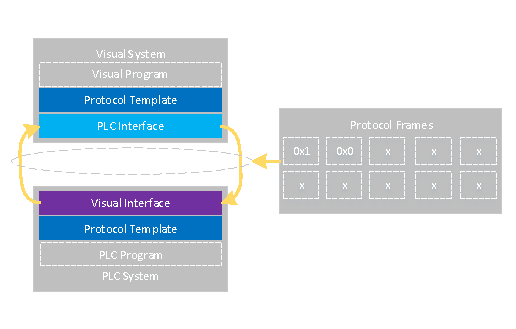
\includegraphics[width=3in]{fig/FlexibleLayer.pdf}
	\caption{ Data Interaction Based on VP Protocol.}
	\label{fig:FlexibleLayer}
\end{figure}
\begin{algorithm}
	\label{alg4}
	\caption{$VLDeframing$}%算法名字
	%\LinesNumbered %要求显示行号
	\KwIn{$PDF$}%输入参数
    $mid \leftarrow$ four bytes start form $PDF$\;
    searchPT ($mid$, $vlt_x$)\;
    CRC16()\;
    $msn \leftarrow$ four bytes start form $PDF+4$\;    
	$CassMemM[vlt_x.mda]\leftarrow$ $msn-8$ bytes start form $PDF+8$\;
	$PDF\leftarrow$ $PDF+msn$\;
\end{algorithm}

\begin{algorithm}
	\label{alg5}
	\caption{$CLDeframing$}%算法名字
	%\LinesNumbered %要求显示行号
	\KwIn{$mid$}%输入参数
	searchPT($mid$, $vlt_x$)\;
	$mda\leftarrow$ $vlt_x.mda$\;
	\For{$i=0$;$i<vlt_x.man$;$i++$}{
		searchPT($vlt_x.mas[i]$, $clt_y$)\;
		$CassMemS[clt_y.apa]\leftarrow$ $clt_y.vfl - 8$ bytes start form $mda+8$\; 
        $mda\leftarrow$ $mda+clt_y.vfl$\;
	}
    clean\;
\end{algorithm}

\begin{algorithm}
	\label{alg6}
	\caption{$ALDeframing$}%算法名字
	%\LinesNumbered %要求显示行号
	\KwIn{$aid$}%输入参数
	searchPT($aid$, $clt_y$)\;
	$ada\leftarrow$ $vlt_x.ada$\;
	\For{$i=0$;$i<clt_y.apn$;$i++$}{
		$CassMemA[CassMemA[ada]]\leftarrow$ $CassMemA[ada+4]$\;
		$ada\leftarrow ada+8$\;
	}
	clean\;
\end{algorithm}


\section{System Operation Mechanism}
\label{Execution}
\subsection{Implementation of Flexible Program and Execution}
The $FL$ contains two parts: $PLC$ interface and visual interface. They interact with each other using the agreed communication protocol which is defined as $CID$ in $HPT$ of $PT$.

The $PLC$ interface is responsible for get parameters of motion control form $VS$ and interact with $ES$. It includes three steps blew.

\textbf{Step 1}: after image processing, the $VS$ extracts the useful data and stores into visual extracted data ($VED$) in which the parameters could be indexed by the $PID$.

\textbf{Step 2}: frame them into $PF$ with the Algorithm \ref{alg1}, \ref{alg2} and \ref{alg3}.

\textbf{Step 3}: transfer the $VCA$ protocol frame to $ePLC$ with the relevant communication protocol in $CID$.

Visual interface is in the $ePLC$ designed to interact with $VS$ and it contains two steps below. 

\textbf{Step 1}: receive $PF$s from $VS$ according the $CID$ in $HPT$.

\textbf{Step 2}: save them in the $ES$. There are two pointers: $PDF$ and $PSP$. $PDF$ points to the address of deframing $PF$ and $PSP$ points to the address of saving $PF$. The $PDF$ will point to the next address of $PF$ if a $PF$ is deframed. After saved the $PF$, the $PSP$ will point to the next new address according the $vfl$ of $PF$. 

  

\begin{figure}
	\centering
	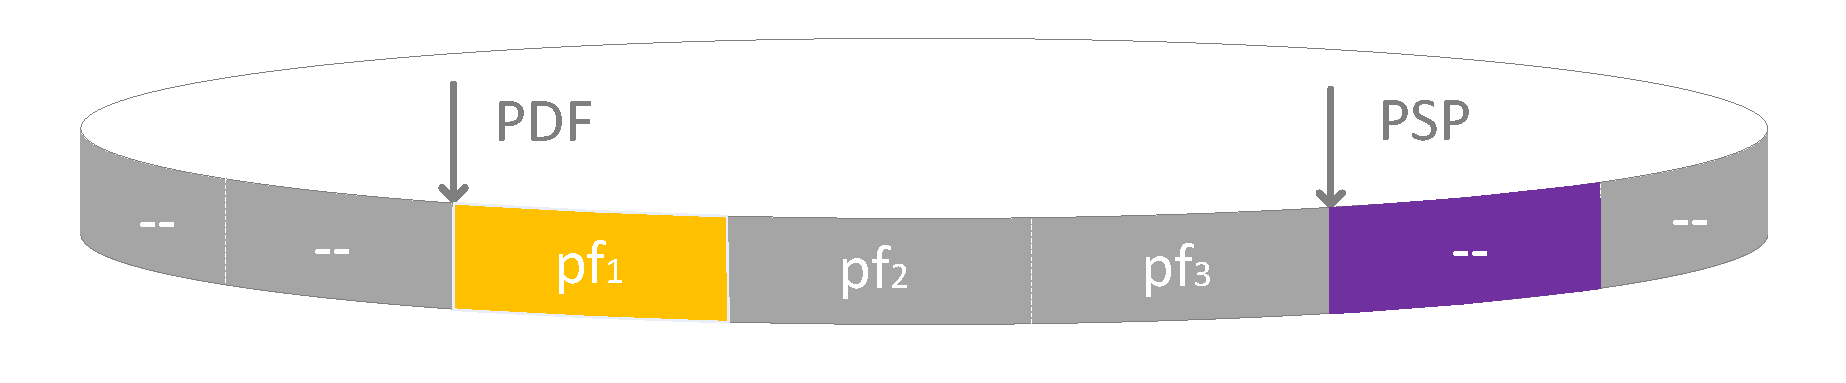
\includegraphics[width=3in]{fig/VisualInterface.pdf}
	\caption{ $PDF$ and $PSP$.}
	\label{fig:VisualInterface}
\end{figure}

%\begin{figure}
%	\centering
%	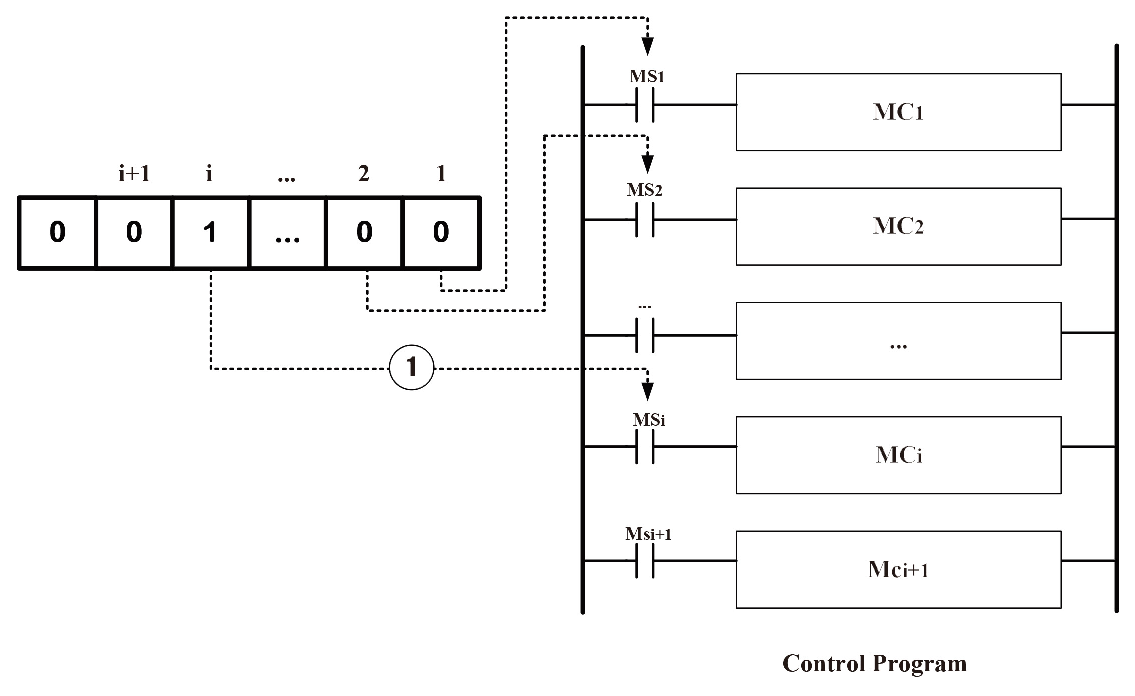
\includegraphics[width=3.5in]{fig/bitdatainM.eps}
%	\caption{Using bit data in the M area to control program module$\textquoteright$s execution}
%	\label{fig:bitdatainM}
%\end{figure}
%%%Fig.11. Using bit data in M area to control program module¡¯s execution.


\subsection{Implementation of Control Program and Execution}
Control program $CP$ is responsible for organizing the modules, executing the logic program, deframing the $PF$ and interacting the data with algorithm program. $CP=\{VLDP,CLDP, IP, LP, PIP\}$, where $CLP$ is the control layer deframe program. $IP$ is the initial program which is used to initialize the data and state. $LP$ is the logic program. $PIP$ is the processor interaction program implemented to transfer and receive data between processors. The implementation of control program is described below.

\textbf{Step 1}: if $PDF!=PSP$, execute the $VLDP$ which means to call Algorithm \ref{alg4}

\textbf{Step 2}: traverse the $LCF$ to check whether there is a module needed to execute. If $\exists$ $\forall$ $lcf_i \in LCF$ is 1, go to step 2.

\textbf{Step 3}: execute the $IP$ to initialize the data and state and then execute the $LP$ to find the called algorithm. If $\exists$ $\forall$ $af_i \in AF$ is 1, go to step 4. 

\textbf{Step 4}: execute the $CLDP$ to call Algorithm \ref{alg5}. 

\textbf{Step 5}: the $\mathcal{P}_{mts}$ is used in $PIP$ to inform the slave processor to receive parameters and start algorithms and clear the relevant $af_i$.   

\textbf{Step 6}: read and process the feedback data form the slave processor. 


%\begin{figure}
%\centering
%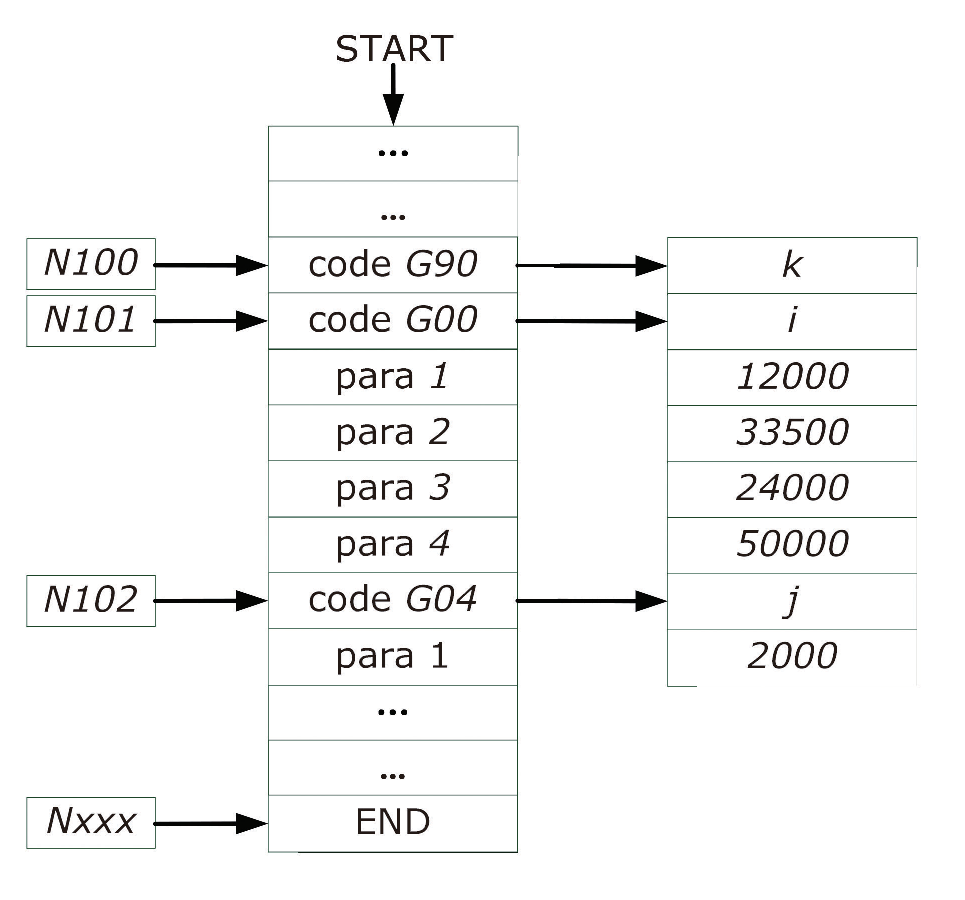
\includegraphics[width=3in]{fig/formatofCNCprogram.eps}
%\caption{The format of ACP program frame after compiling}
%\label{fig:formatofCNCprogram}
%\end{figure}
%%%Fig.8. The format of ACP program frame after compiling.




%%%Fig.9. The schematic of delivering ACP instruction parameters from ACPDD to ACPPSD

%\begin{figure}
%	\centering
%	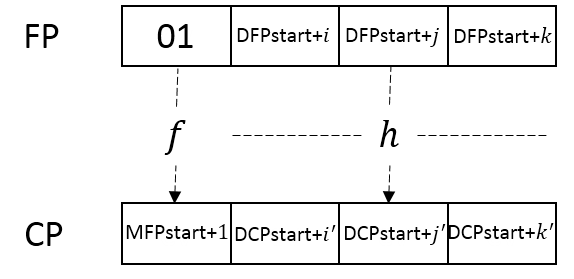
\includegraphics[width=2.5in]{fig/compilation.png}
%	\caption{ The compilation from flexible program to control program}
%	\label{fig:compilation}
%\end{figure}

%\begin{figure}
%	\centering
%	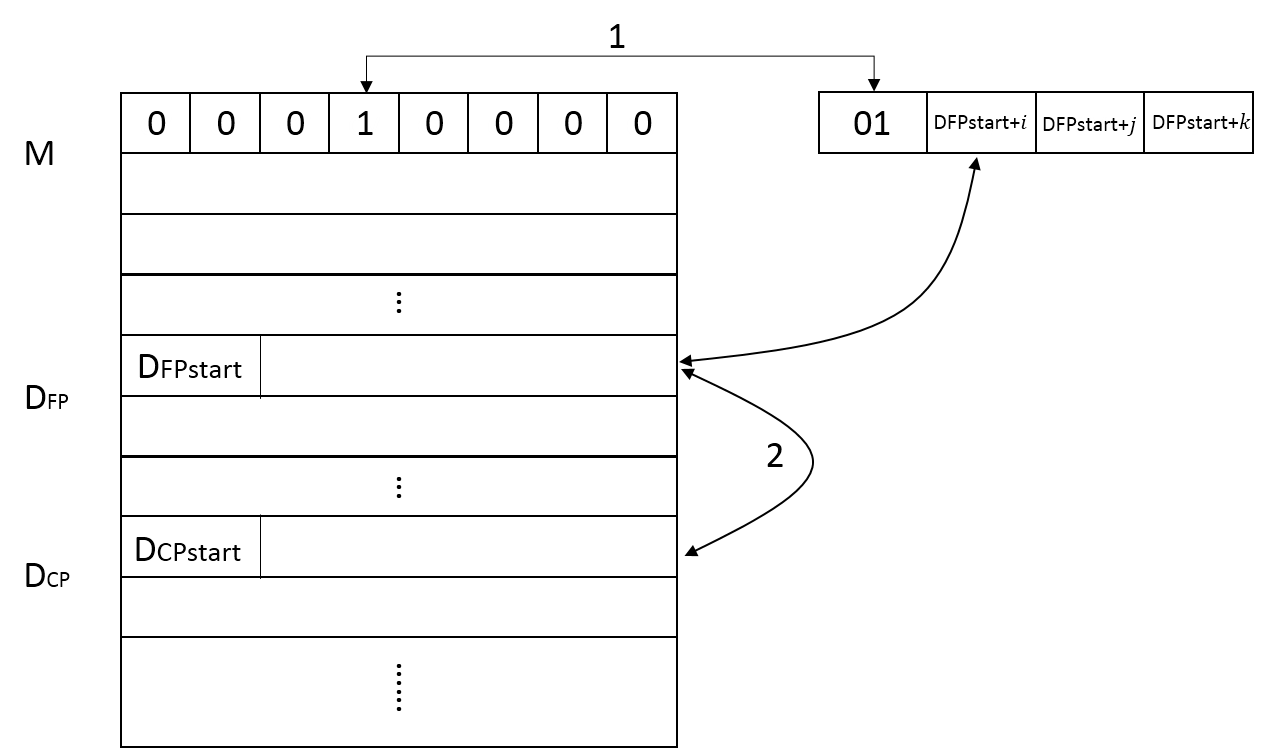
\includegraphics[width=2.5in]{fig/DataTransfer.png}
%	\caption{ The compilation from flexible program to control program}
%	\label{fig:DataTransfer}
%\end{figure}

%\begin{figure}
%	\centering
%	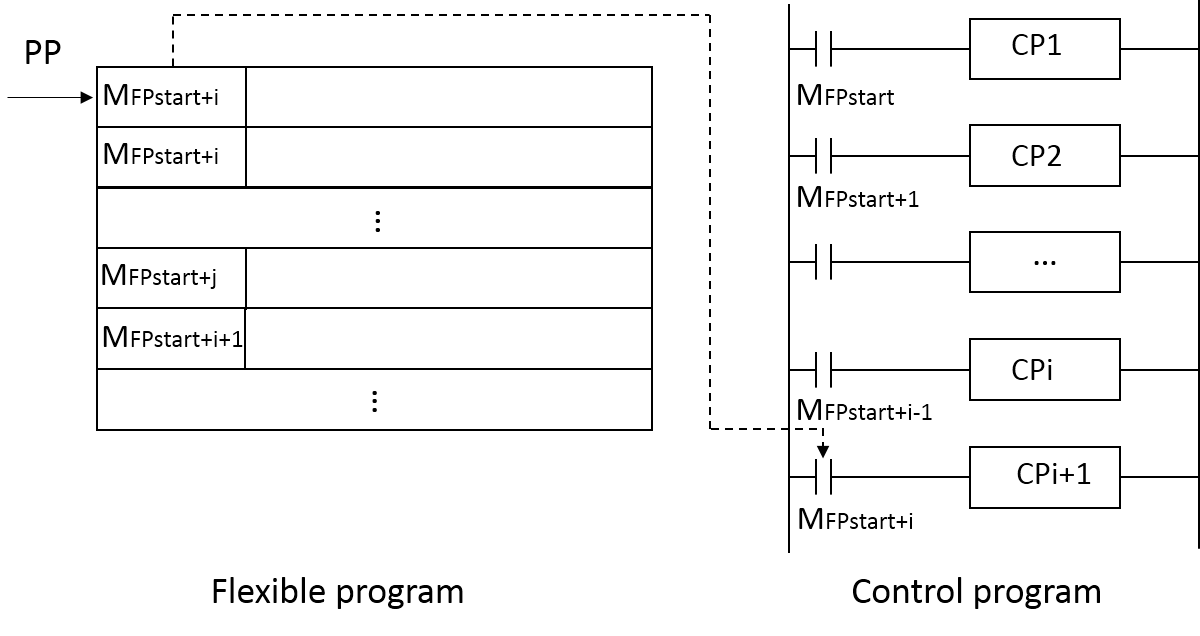
\includegraphics[width=3in]{fig/execution.png}
%	\caption{ The execution OF flexible program}
%	\label{fig:execution}
%\end{figure}

\subsection{Implementation and Execution of Algorithm Program }
The Algorithm Program ($AP$) is in $EL$. $AP=\{\mathcal{P}_{stm}, AS, ALDP\}$, where $\mathcal{P}_{stm}$ feeds back data to master processor, $AS$ contains all algorithms and $ALDP$ deframe the $AL$ frame. The execution of algorithm program is introduced below.

\textbf{Step 1}: traverse the $LCF$ to check whether there is a algorithm needed to execute. If $\exists$ $\forall$ $af_i \in AF$ is 1, go to step 2.

\textbf{Step 2}: ALDP is executed to call Algorithm \ref{alg5}. The parameters are transfered to correlative $as_i$.

\textbf{Step 3}: $as_i$ is executed and uses the $\mathcal{P}_{stm}$ to feed back data to the master processor. 

\subsection{Execution of Threads}
 Commonly, threads in master processor and in slave processors execute separately according to their priority and the interaction between control thread and algorithm threads occurs when using $\mathcal{P}_{mts}$ and $\mathcal{P}_{mts}$. 
 
 Visual thread consists of the following units.
 
 \textbf{$V_1$}}: receive $PF$ from $VS$ with the agreed communication protocol.
 
 \textbf{$V_2$}: check $PF$ and store it into $VD$. 
 
 \textbf{$V_3$}: call Algorithm \ref{alg4} to deframe the $PF$ and saved the $cdata$ into $LCD$.
 
 Basic execution units of control thread are shown as follows:

\textbf{$C_{1}$}: start a module and initial it.

\textbf{$C_{2}$}: run logic program. 

\textbf{$C_{3}$}: call Algorithm \ref{alg5} to deframe control frame.

\textbf{$C_{4}$}: transfer data to slave processor by $\mathcal{P}_{mts}$.

\textbf{$C_{5}$}: deal with the feedback data.

\textbf{$C_{6}$}: end the module.

Motion thread contains the following basic execution units:

\textbf{$M_{1}$}: Start a algorithm.

\textbf{$M_{2}$}: Call Algorithm \ref{alg6} to deframe the algorithm frame.

\textbf{$M_{3}$}: Execute the algorithm.

\textbf{$M_{4}$}: Feedback the data to master processor by $\mathcal{P}_{stm}$.

\textbf{$M_{5}$}: End the algorithm.

The threads execute as shown in Fig. \ref{fig:threadExecution}. Visual thread ($VT$) continuously executes the unit $V1$ if there exits $PF$ from $VS$, executes unit $V2$ to store the $PF$ into $VD$ at the address of $PSP$ and execute $V3$ to deframe $PF$ at the address of $PDF$ and store its $cdata$ into $LCD$ and $\mathcal{S}_1 {cdf_i}$.
The control thread ($CT$) traverses $LCF$, finds $\exists \mathcal{J}_1 {lcf_i}$ and then executes the unit $C1$, executes unit $C_2$. If find a required execution algorithm and $\exists$ its $\mathcal{J}_1 {mdf_j}$ then $CT$ starts unit $C3$ to deframe the control frame and then runs unit $C4$ and inform algorithm thread ($AT$) to execute $M_1$ unit. Next, $AT$ executes unit $M2$ transferring data from $SMD$ to $AD$. After that, the unit $M3$ is executed. During the running of algorithm, the unit $M4$ is continuously executed to feed data back to $CT$, meanwhile $CT$ will execute unit $C5$ to response it until the execution of $M5$ and no other executed algorithms neither. During the running of the module, if the $VT$ receives new $PF$ and $CT$ finds $\exists \mathcal{J}_1 {cdf_i}$, $CT$ will execute unit $C_3$ and $C_4$ again. Next, the $VT$ will run unit $M_2$ to update the parameters. If the $MT$ finished all algorithms, then $CT$ will run unit $C_6$ to finished the module and continue to traverse the $LCF$ to find another required execution module.   

\begin{figure}
	\centering
	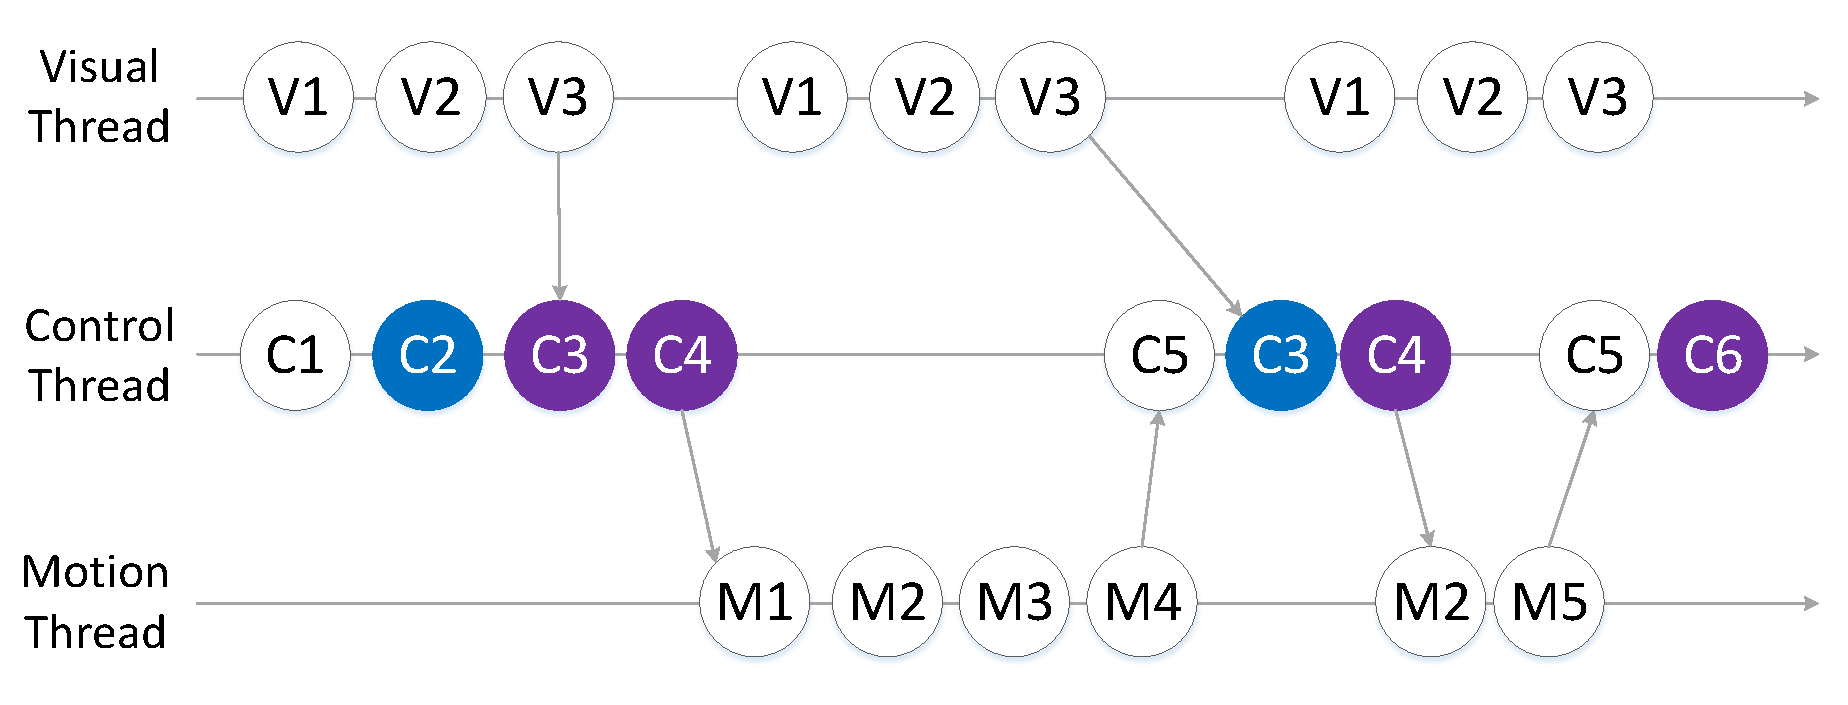
\includegraphics[width=3in]{fig/ThreadExecution.pdf}
	\caption{ Visual servo control system}
	\label{fig:threadExecution}
\end{figure}

\section{Case Analysis}
\label{Case}
In this section, we introduce two scenarios of the proposed $VCA$ protocol based integration method in ePLC. With the $VCA$ protocol, users only need to code additional algorithms and change the $PT$ when the scenario of visual servo system is changed. 
\subsection{Case 1 Binocular Catching Robot}
\begin{figure}
	\centering
	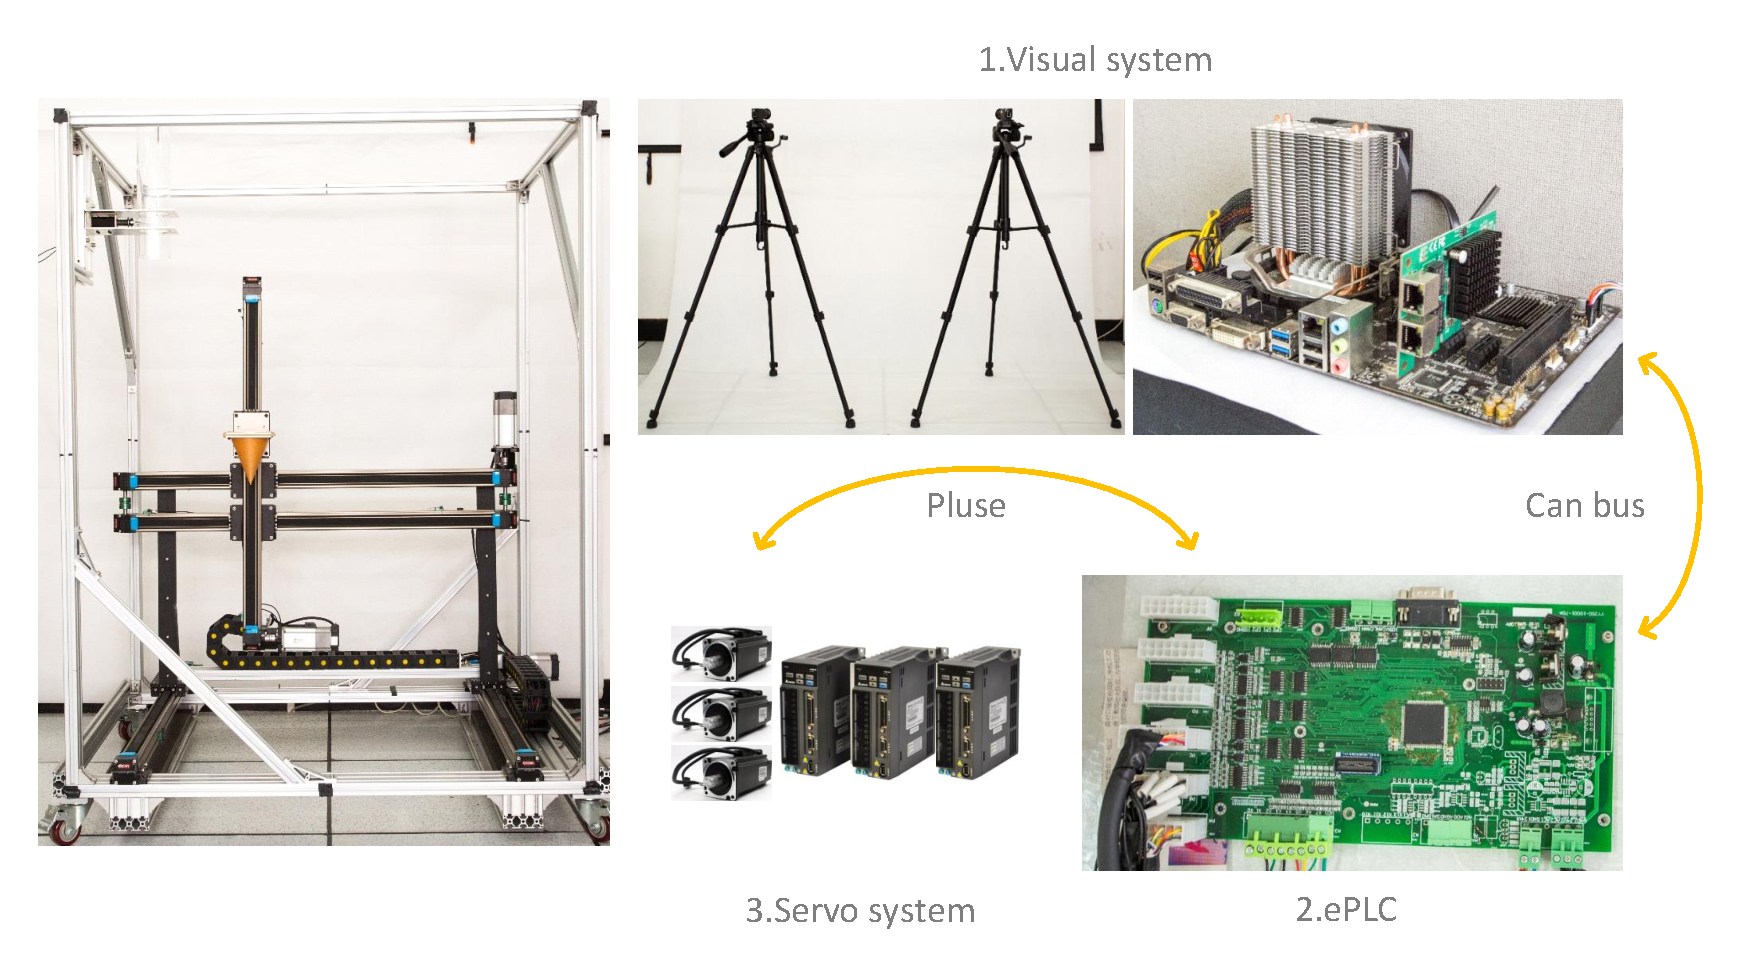
\includegraphics[width=3in]{fig/robot.pdf}
	\caption{ Visual servo control system}
	\label{fig:robot}
\end{figure}
As shown in Fig. \ref{fig:robot}, the binocular catching robot adopts two cameras to judge the position of the ball. Through sending the continuously parameters to $ePLC$ to adjust the position of the robot. Finally, the robot will catch the ball. The cameras is xxx, the visual system is xxx, and the $ePLC$ is XXX. $ePLC$ uses tht TI F28M35 chip with two cores: ARM Cortex M3 and TI C28x, which contains a shared RAM. The servo driver and motor are xxx and xxx respectively. 
\subsubsection{Design of $PT$}

\begin{table}
	\scriptsize \caption{$PT$ of binocular catching robot}
	\label{table:PTofRobot}
	\begin{center}
		\renewcommand{\arraystretch}{1.4}
		\setlength\tabcolsep{3pt}
		\begin{tabular}{|c|c|c|c|c|c|c|}
			\hline
			CID  & TDA   &xxx &xxx& xxx  &xxx &xxx \\
			\hline
			0X03000001&0x00&& &&&\\
			\hline
			MID   & MAN  & MSF  & MDF  &MAS1    & MAS2&xxx\\
			\hline
			0X02000001 & 1  & 0X400  & 0X600   &0X02000001   & &\\
			\hline
			AID  & APN  & AF  &ADA  &APS1   &APS2&APS3\\
			\hline
			0X02000001 & 0X9  & 0X14A  &0x1F4000  &0X1   &0X2 &0X3\\
			\hline
			APS4  & APS5  & APS6  &APS7   &APS8   &APS9&xxx\\
			\hline
			0X4  & 0X5  & 0X6  &0x7  &0X8  &0X9&\\
			\hline
		\end{tabular}
	\end{center}
\end{table}

\subsubsection{Design of Program}

\subsubsection{Result}



\begin{figure}
	\centering
	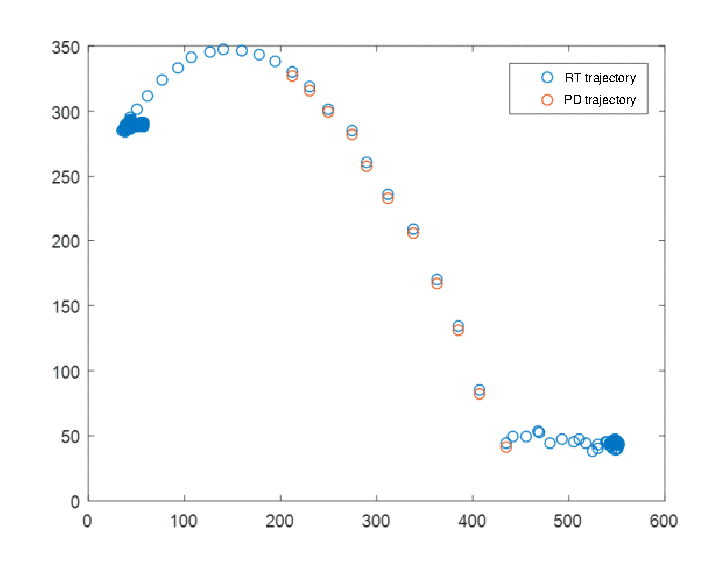
\includegraphics[width=3.5in]{fig/PFofRobot.pdf}
	\caption{ The execution OF flexible program}
	\label{fig:settingexecutionbitinACPTD}
\end{figure}

\subsection{Case 2 Winding Machine with Visual System}

\subsubsection{Design of $PT$}

\subsubsection{Design of Program}

\subsubsection{Result}
\begin{figure}
	\centering
	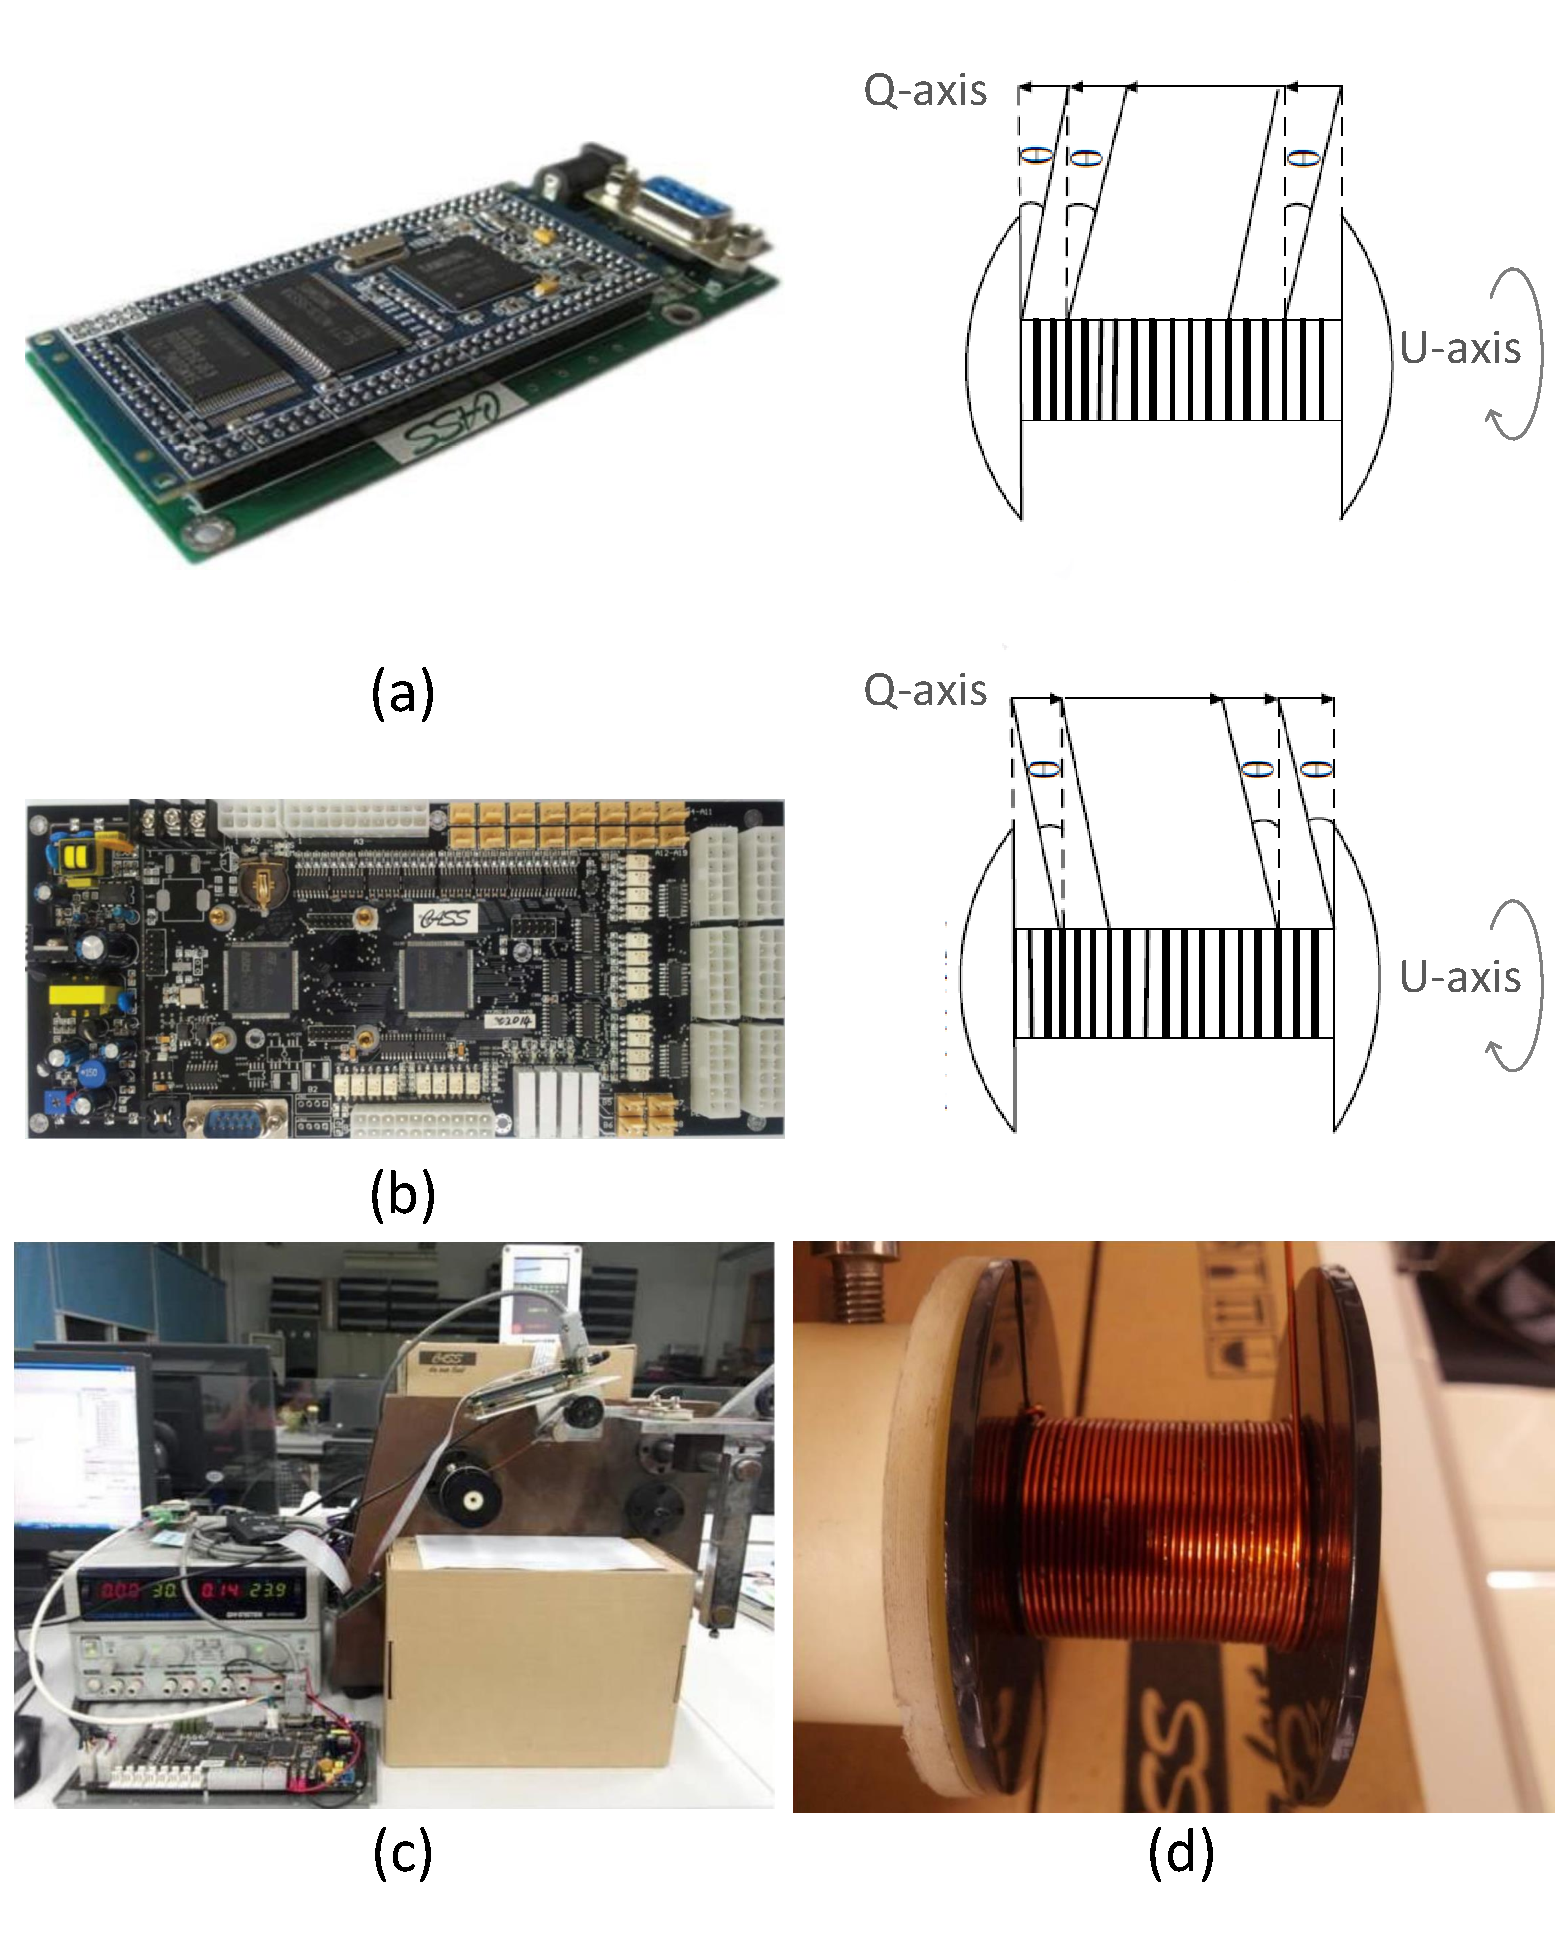
\includegraphics[width=3in]{fig/Winding.pdf}
	\caption{ Winding machine Based on Visual System}
	\label{fig:Winding}
\end{figure}
\section{Conclusion}
\label{conclusion}

In the further research, we will implement a uniform development method of the visual servo control in ePLC.

\ifCLASSOPTIONcaptionsoff
  \newpage
\fi



% trigger a \newpage just before the given reference
% number - used to balance the columns on the last page
% adjust value as needed - may need to be readjusted if
% the document is modified later
%\IEEEtriggeratref{8}
% The "triggered" command can be changed if desired:
%\IEEEtriggercmd{\enlargethispage{-5in}}

% references section

% can use a bibliography generated by BibTeX as a .bbl file
% BibTeX documentation can be easily obtained at:
% http://www.ctan.org/tex-archive/biblio/bibtex/contrib/doc/
% The IEEEtran BibTeX style support page is at:
% http://www.michaelshell.org/tex/ieeetran/bibtex/
%\bibliographystyle{IEEEtran}
% argument is your BibTeX string definitions and bibliography database(s)
%\bibliography{IEEEabrv,../bib/paper}
%
% <OR> manually copy in the resultant .bbl file
% set second argument of \begin to the number of references
% (used to reserve space for the reference number labels box)

\bibliographystyle{IEEEtran}
\bibliography{reference}

% biography section
%
% If you have an EPS/PDF photo (graphicx package needed) extra braces are
% needed around the contents of the optional argument to biography to prevent
% the LaTeX parser from getting confused when it sees the complicated
% \includegraphics command within an optional argument. (You could create
% your own custom macro containing the \includegraphics command to make things
% simpler here.)
%\begin{IEEEbiography}[{\includegraphics[width=1in,height=1.25in,clip,keepaspectratio]{mshell}}]{Michael Shell}
% or if you just want to reserve a space for a photo:

%\begin{IEEEbiography}[{\includegraphics[width=1in,height=1.25in,clip,keepaspectratio]{fig/Author_HuifengWu.eps}}]{Huifeng Wu} received the Ph.D. degree in computer science and technology from Zhejiang university, Hangzhou, China, in 2006. He is currently a professor in the institute of intelligent and software Technology, Hangzhou Dianzi University. His research interests include software development methods and tools, software architecture, embedded system, intelligent control \& automation.
%	
%\end{IEEEbiography}
%\begin{IEEEbiography}[{\includegraphics[width=1in,height=1.25in,clip,keepaspectratio]{fig/Author_YiYan.eps}}]{Yi Yan} received B.S. in automatic control engineering form Zhejiang Sci-Tech University in 1984, M.S. in computer engineering from Beijing University of Postal Telecommunications in 1990. Currently he is the director and full professor in institute of intelligent and software Technology, Hangzhou Dianzi University. His research interests include embedded system, advanced manufacturing system, intelligent control \& automation, and intelligent instruments.
%	
%	
%\end{IEEEbiography}
%\begin{IEEEbiography}[{\includegraphics[width=1in,height=1.25in,clip,keepaspectratio]{fig/Author_DanfengSun.eps}}]{Danfeng Sun} received M.S. in computer architecture from Hangzhou DianZi University in 2011. He is currently a research assistant in the Institute of Industrial Internet, Hangzhou DianZi University. His research interests include embeded system, motion control and IIoT.
%\end{IEEEbiography}
%\begin{IEEEbiography}[{\includegraphics[width=1in,height=1.25in,keepaspectratio,angle=-90]{fig/Author_ReneSimon.eps}}]{Rene Simon} obtained a doctor of engineering at the Otto-von-Guericke University Magdeburg in 2001. He is Professor of Control Systems at the Department of Automation and Computer Sciences, Harz University of Applied Sciences, Wernigerode, Germany. His major research fields include engineering of automation systems, especially industrial controllers. He is chairman of PLCopen and project leader IEC 61131-10 Ed. 1.0.
%\end{IEEEbiography}



% insert where needed to balance the two columns on the last page with
% biographies
%\newpage


% You can push biographies down or up by placing
% a \vfill before or after them. The appropriate
% use of \vfill depends on what kind of text is
% on the last page and whether or not the columns
% are being equalized.

%\vfill

% Can be used to pull up biographies so that the bottom of the last one
% is flush with the other column.
%\enlargethispage{-5in}



% that's all folks
\end{document}


